\chapter{Complete Link Budget Analysis}
\label{ch:linkbudget}

\begin{nontechnical}
\textbf{Link budget is like a financial budget for radio power}---you start with transmit power, add gains, subtract losses, and see if there's enough ``money'' (signal) left at the receiver.

\textbf{The fundamental question:} ``If I transmit from HERE to THERE, will the receiver get enough signal?''

\textbf{Simple accounting:}
\begin{itemize}
\item \textbf{START:} Transmit power (WiFi: 20~dBm, Satellite: 50~dBm)
\item \textbf{ADD:} Antenna gains (WiFi: +2~dB, Satellite dish: +40~dB)
\item \textbf{SUBTRACT:} Path loss (50~m WiFi: -74~dB, GEO satellite: -206~dB!)
\item \textbf{SUBTRACT:} Other losses (walls: -5~dB each, rain: -10~dB)
\item \textbf{END:} Received power---must be stronger than noise floor!
\end{itemize}

\textbf{Example---WiFi at home:}

Start with 20~dBm, add 2~dB antenna gain = 22~dBm radiated. Lose 74~dB in free space over 50~m, lose 10~dB through 2 walls. Receive -62~dBm. Noise floor is -90~dBm. Result: 28~dB signal-to-noise ratio---excellent!

\textbf{Satellite TV example:}

Satellite transmits 50~dBm with 35~dB antenna gain. Lose 206~dB over 36,000~km! Your dish adds 35~dB gain. Receive -86~dBm. Noise floor -100~dBm. Result: 14~dB SNR---just enough!

\textbf{The margin is everything:} 10--20~dB margin = robust link. 3--5~dB margin = risky (rain will kill it). Negative margin = link fails!

\textbf{Fun fact:} Voyager 1 transmits 23~W from 24 billion kilometers away. Received power at Earth: $10^{-16}$~watts. Only 70-meter dishes with meticulous link budgets can hear it!
\end{nontechnical}

\section{Overview}

\textbf{Link budget analysis} is the systematic accounting of all power gains and losses in a wireless communication system from transmitter to receiver. It answers the fundamental engineering question: \emph{``Will this link work?''}

The analysis computes the received signal power and compares it to the minimum required signal level (receiver sensitivity) to determine if the link can sustain reliable communication.

\begin{keyconcept}
A positive link margin indicates the link will function reliably. The margin magnitude determines robustness against fading, interference, and environmental degradation. Industry practice requires 10--30~dB margin depending on reliability requirements.
\end{keyconcept}

\textbf{Core equation:}
\begin{equation}
\label{eq:link_budget_basic}
P_r = P_t + G_t - L_{\text{path}} + G_r - L_{\text{misc}}
\end{equation}
where:
\begin{itemize}
\item $P_r$ = received power (dBm)
\item $P_t$ = transmitted power (dBm)
\item $G_t$, $G_r$ = transmit and receive antenna gains (dBi)
\item $L_{\text{path}}$ = path loss (dB)
\item $L_{\text{misc}}$ = miscellaneous losses (cables, connectors, etc.) (dB)
\end{itemize}

\textbf{Link closure criterion:}
\begin{equation}
\label{eq:link_margin}
M = P_r - P_{\text{min}} > 0
\end{equation}
where $M$ is the link margin (dB) and $P_{\text{min}}$ is the receiver sensitivity (dBm).

\section{End-to-End System Model}

A wireless communication link consists of three primary domains: transmitter, propagation channel, and receiver.

\subsection{System Block Diagram}

\begin{center}
\begin{tikzpicture}[
  block/.style={rectangle, draw, minimum width=2.5cm, minimum height=1.2cm, font=\sffamily\small, align=center},
  loss/.style={rectangle, draw, dashed, minimum width=2.5cm, minimum height=1.2cm, font=\sffamily\small, align=center, fill=black!5},
  node distance=3cm,
  font=\small
]

% Transmitter chain
\node[block] (txamp) {TX\\Power Amp\\$P_t$};
\node[block, right of=txamp] (txant) {TX\\Antenna\\$G_t$};

% Channel
\node[loss, right of=txant, node distance=4cm] (channel) {Propagation\\Channel\\$-L_{\text{path}}$};

% Receiver chain
\node[block, right of=channel, node distance=4cm] (rxant) {RX\\Antenna\\$G_r$};
\node[block, right of=rxant] (rxamp) {LNA \&\\Receiver\\NF};

% Signal flow
\draw[->,thick] (txamp) -- node[above,font=\scriptsize] {$P_t$~dBm} (txant);
\draw[->,thick] (txant) -- node[above,font=\scriptsize] {EIRP} (channel);
\draw[->,thick] (channel) -- node[above,font=\scriptsize] {$-L$~dB} (rxant);
\draw[->,thick] (rxant) -- node[above,font=\scriptsize] {$P_r$~dBm} (rxamp);

% Loss annotations
\node[below=0.8cm of txant, font=\scriptsize] {$-L_{\text{TX}}$~dB};
\node[below=0.8cm of rxant, font=\scriptsize] {$-L_{\text{RX}}$~dB};

\end{tikzpicture}
\end{center}

Power flows from transmitter through the channel to the receiver, accumulating gains and losses at each stage.

\section{Mathematical Description}

\subsection{Link Budget Components}

\subsubsection{Transmitter Power}

The \textbf{transmitted power} $P_t$ is the RF power delivered to the transmit antenna after accounting for power amplifier output and transmission line losses:

\begin{equation}
\label{eq:tx_power}
P_t = P_{\text{amp}} - L_{\text{TX}}
\end{equation}
where:
\begin{itemize}
\item $P_{\text{amp}}$ = power amplifier output (dBm)
\item $L_{\text{TX}}$ = transmitter losses---cables, filters, circulators (dB)
\end{itemize}

\textbf{Example:} WiFi router with PA output 20~dBm and cable loss 0.5~dB yields $P_t = 20 - 0.5 = 19.5$~dBm.

\subsubsection{Transmit Antenna Gain and EIRP}

The transmit antenna provides directional gain $G_t$ (dBi) relative to an isotropic radiator. The combination of transmit power and antenna gain defines the \textbf{Effective Isotropic Radiated Power (EIRP)}:

\begin{equation}
\label{eq:eirp}
\text{EIRP} = P_t + G_t
\end{equation}
where:
\begin{itemize}
\item EIRP = equivalent isotropic radiated power (dBm or dBW)
\item $G_t$ = transmit antenna gain (dBi)
\end{itemize}

\textbf{Example:} $P_t = 19.5$~dBm with $G_t = 2$~dBi yields EIRP = $21.5$~dBm.

\begin{warningbox}
Regulatory bodies (FCC, ETSI, etc.) impose strict EIRP limits to prevent interference. For example, FCC Part 15 limits 2.4~GHz ISM band EIRP to 36~dBm (4~W). Exceeding these limits risks fines and equipment seizure.
\end{warningbox}

\subsubsection{Free-Space Path Loss}

\textbf{Free-space path loss (FSPL)} represents the attenuation of electromagnetic waves due to spherical spreading in free space, independent of absorption or obstacles:

\begin{equation}
\label{eq:fspl_fundamental}
L_{\text{FSPL}} = \left(\frac{4\pi d f}{c}\right)^2
\end{equation}
where:
\begin{itemize}
\item $d$ = distance between transmitter and receiver (m)
\item $f$ = frequency (Hz)
\item $c = 3 \times 10^8$~m/s = speed of light
\end{itemize}

In logarithmic form (more practical for link budgets):
\begin{equation}
\label{eq:fspl_db}
L_{\text{FSPL}} = 20\log_{10}(d) + 20\log_{10}(f) + 20\log_{10}\left(\frac{4\pi}{c}\right)
\end{equation}

\textbf{Practical formula} with distance in kilometers and frequency in MHz:
\begin{equation}
\label{eq:fspl_practical}
L_{\text{FSPL}} = 32.45 + 20\log_{10}(d_{\text{km}}) + 20\log_{10}(f_{\text{MHz}})
\end{equation}

\textbf{Example:} WiFi at 2.4~GHz over 100~m:
\begin{equation}
L_{\text{FSPL}} = 32.45 + 20\log_{10}(0.1) + 20\log_{10}(2400) = 32.45 - 20 + 67.6 = 80~\text{dB}
\end{equation}

\textbf{Key insight:} FSPL increases 20~dB per decade of distance and 20~dB per decade of frequency. Doubling distance or frequency adds 6~dB loss.

For detailed FSPL derivation, see Chapter~\ref{ch:fspl}.

\subsubsection{Atmospheric Absorption}

Oxygen and water vapor in the atmosphere absorb electromagnetic energy, particularly at millimeter-wave frequencies. The specific \textbf{attenuation coefficient} $\gamma_{\text{atm}}$ depends on frequency:

\begin{equation}
\label{eq:atm_loss}
L_{\text{atm}} = \gamma_{\text{atm}} \cdot d_{\text{path}}
\end{equation}
where:
\begin{itemize}
\item $\gamma_{\text{atm}}$ = attenuation per unit distance (dB/km)
\item $d_{\text{path}}$ = path length through atmosphere (km)
\end{itemize}

\textbf{Representative values (zenith, sea level):}

\begin{center}
\begin{tabular}{@{}lll@{}}
\toprule
Frequency & $\gamma_{\text{atm}}$ (dB/km) & Notes \\
\midrule
$< 10$~GHz & $< 0.01$ & Negligible \\
22.2~GHz & 0.2 & H$_2$O resonance \\
60~GHz & 15 & O$_2$ resonance (peak) \\
120~GHz & 2 & Secondary O$_2$ line \\
183~GHz & 5 & H$_2$O line \\
\bottomrule
\end{tabular}
\end{center}

\textbf{Example:} Ka-band satellite at 20~GHz, $5°$ elevation angle (path length $\approx 11$~km): $L_{\text{atm}} \approx 0.05 \times 11 = 0.55$~dB.

\subsubsection{Rain Attenuation}

Rain is the dominant propagation impairment for satellite links above 10~GHz. The \textbf{ITU-R rain attenuation model} relates specific attenuation to rain rate:

\begin{equation}
\label{eq:rain_specific}
\gamma_R = k \cdot R^{\alpha}
\end{equation}
where:
\begin{itemize}
\item $\gamma_R$ = specific rain attenuation (dB/km)
\item $R$ = rain rate (mm/hr)
\item $k$, $\alpha$ = frequency-dependent coefficients (from ITU-R P.838)
\end{itemize}

\textbf{Total rain attenuation:}
\begin{equation}
\label{eq:rain_total}
L_{\text{rain}} = \gamma_R \cdot d_{\text{eff}}
\end{equation}
where $d_{\text{eff}}$ is the effective path length through rain (typically 2--5~km).

\textbf{Example:} Ku-band at 12~GHz, heavy rain (25~mm/hr), 4~km path. From ITU tables: $k = 0.0188$, $\alpha = 1.217$.
\begin{equation}
\gamma_R = 0.0188 \times 25^{1.217} = 1.2~\text{dB/km} \quad \Rightarrow \quad L_{\text{rain}} = 1.2 \times 4 = 4.8~\text{dB}
\end{equation}

\begin{calloutbox}{Link Availability Design}
For 99\% availability, design for rain rate exceeded 1\% of time: 12~mm/hr (temperate), 42~mm/hr (tropical). For 99.9\% availability, add 5--10~dB additional rain margin.
\end{calloutbox}

\subsubsection{Additional Propagation Effects}

Real-world channels introduce additional losses beyond free-space propagation:

\begin{center}
\begin{tabular}{@{}lll@{}}
\toprule
Effect & Typical Loss & Applicability \\
\midrule
Ionospheric scintillation & 1--20~dB & L-band satellite, equatorial \\
Tropospheric scintillation & 0.5--2~dB & Low elevation, $>10$~GHz \\
Polarization mismatch & 0--$\infty$~dB & Misalignment, Faraday rotation \\
Multipath fading & 10--30~dB & Mobile, urban NLOS \\
Foliage loss & 0.3--1~dB/m & Trees, VHF/UHF \\
Building penetration & 5--20~dB & Indoor \\
\bottomrule
\end{tabular}
\end{center}

\textbf{Total path loss:}
\begin{equation}
\label{eq:total_path_loss}
L_{\text{total}} = L_{\text{FSPL}} + L_{\text{atm}} + L_{\text{rain}} + L_{\text{other}}
\end{equation}

\subsubsection{Receiver Antenna and System}

The receive antenna provides gain $G_r$ (dBi) by the same reciprocity principles as the transmit antenna. Typical values:
\begin{itemize}
\item Omnidirectional (WiFi laptop): 0~dBi
\item Yagi (TV, point-to-point): 10--15~dBi
\item Parabolic dish (satellite): 30--60~dBi
\end{itemize}

\textbf{Receiver line losses} $L_{\text{RX}}$ include:
\begin{itemize}
\item Cable loss: 0.5--3~dB (depends on length, frequency, cable type)
\item Connector loss: 0.1--0.5~dB per connector
\item Filter insertion loss: 0.5--2~dB
\item Circulator/duplexer loss: 0.5--1~dB
\end{itemize}

\textbf{Received signal power:}
\begin{equation}
\label{eq:received_power}
P_r = \text{EIRP} - L_{\text{total}} + G_r - L_{\text{RX}}
\end{equation}

\subsubsection{Receiver Sensitivity}

The \textbf{receiver sensitivity} $P_{\text{min}}$ is the minimum signal power required to achieve acceptable performance (target bit error rate). It is determined by thermal noise, receiver noise figure, and required signal-to-noise ratio:

\begin{equation}
\label{eq:sensitivity}
P_{\text{min}} = N_0 + 10\log_{10}(B) + \text{NF} + \text{SNR}_{\text{req}} + L_{\text{impl}}
\end{equation}
where:
\begin{itemize}
\item $N_0 = -174$~dBm/Hz = thermal noise spectral density at 290~K
\item $B$ = signal bandwidth (Hz)
\item NF = receiver noise figure (dB)
\item $\text{SNR}_{\text{req}}$ = required signal-to-noise ratio for target BER (dB)
\item $L_{\text{impl}}$ = implementation losses---quantization, imperfect synchronization (typically 1--3~dB)
\end{itemize}

\textbf{Example:} WiFi 802.11n, 20~MHz channel, QPSK 1/2:
\begin{equation}
P_{\text{min}} = -174 + 10\log_{10}(20 \times 10^6) + 6 + 5 + 2 = -174 + 73 + 13 = -88~\text{dBm}
\end{equation}

\section{Complete Link Budget Equation}

The complete link budget combines all gains and losses from transmitter to receiver:

\begin{equation}
\label{eq:link_budget_complete}
P_r = P_t + G_t - L_{\text{total}} + G_r - L_{\text{RX}}
\end{equation}

Substituting EIRP and expanding $L_{\text{total}}$:
\begin{equation}
\label{eq:link_budget_expanded}
P_r = \text{EIRP} - L_{\text{FSPL}} - L_{\text{atm}} - L_{\text{rain}} - L_{\text{other}} + G_r - L_{\text{RX}}
\end{equation}

\textbf{Link margin} quantifies robustness:
\begin{equation}
\label{eq:margin}
M = P_r - P_{\text{min}}
\end{equation}

\textbf{Design guidelines:}
\begin{itemize}
\item $M < 0$~dB: Link fails
\item $M = 0$--5~dB: Marginal (high outage probability)
\item $M = 5$--10~dB: Adequate for fixed links
\item $M = 10$--20~dB: Good for mobile/fading channels
\item $M = 20$--30~dB: Excellent (high availability, robust to interference)
\end{itemize}

\subsection{Link Budget Flow Diagram}

\begin{center}
\begin{tikzpicture}[
  box/.style={rectangle, draw, minimum width=4cm, minimum height=0.8cm, font=\sffamily\small, align=center},
  node distance=1.2cm,
  font=\small
]

\node[box, fill=green!20] (eirp) {EIRP\\$P_t + G_t$};
\node[box, fill=red!20, below=of eirp] (fspl) {$-$ FSPL\\$32.45 + 20\log d + 20\log f$};
\node[box, fill=red!20, below=of fspl] (atm) {$-$ Atmospheric Loss\\$\gamma_{\text{atm}} \cdot d$};
\node[box, fill=red!20, below=of atm] (rain) {$-$ Rain Attenuation\\$k R^{\alpha} \cdot d_{\text{eff}}$};
\node[box, fill=red!20, below=of rain] (other) {$-$ Other Losses\\Multipath, penetration};
\node[box, fill=green!20, below=of other] (rxgain) {$+$ RX Antenna Gain\\$G_r$};
\node[box, fill=red!20, below=of rxgain] (rxloss) {$-$ RX Line Losses\\$L_{\text{RX}}$};
\node[box, fill=blue!20, below=of rxloss] (pr) {\textbf{Received Power}\\$P_r$};

\draw[->,thick] (eirp) -- (fspl);
\draw[->,thick] (fspl) -- (atm);
\draw[->,thick] (atm) -- (rain);
\draw[->,thick] (rain) -- (other);
\draw[->,thick] (other) -- (rxgain);
\draw[->,thick] (rxgain) -- (rxloss);
\draw[->,thick] (rxloss) -- (pr);

\node[right=0.5cm of pr, box, fill=orange!20, minimum width=3cm] (sens) {Sensitivity\\$P_{\text{min}}$};
\node[below=0.5cm of sens, box, fill=yellow!30, minimum width=3cm] (margin) {\textbf{Margin}\\$M = P_r - P_{\text{min}}$};

\draw[->,thick,dashed] (pr.east) -- (sens.west);
\draw[->,thick] (sens) -- (margin);

\end{tikzpicture}
\end{center}

Gains (green) increase power, losses (red) decrease power. The margin (yellow) determines link viability.

\subsection{Margin Calculation Illustration}

The link margin represents the safety buffer above the minimum required signal level:

\begin{center}
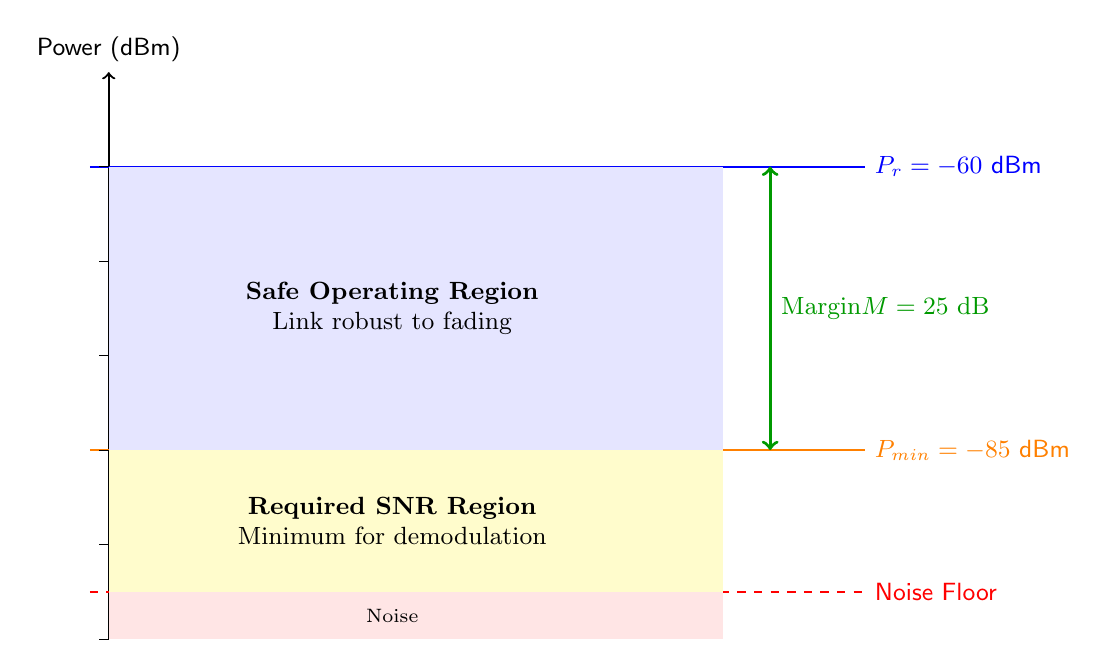
\begin{tikzpicture}[
  font=\small,
  scale=1.2
]

% Power scale (vertical axis)
\draw[thick,->] (0,0) -- (0,6) node[above,font=\sffamily\small] {Power (dBm)};

% Horizontal lines for different power levels
\draw[thick,blue] (-0.2,5) -- (8,5) node[right,font=\sffamily\small] {$P_r = -60$~dBm};
\draw[thick,orange] (-0.2,2) -- (8,2) node[right,font=\sffamily\small] {$P_{\text{min}} = -85$~dBm};
\draw[thick,red,dashed] (-0.2,0.5) -- (8,0.5) node[right,font=\sffamily\small] {Noise Floor};

% Margin bracket
\draw[<->,very thick,green!60!black] (7,2) -- (7,5) node[midway,right] {Margin\\$M = 25$~dB};

% Shaded regions
\fill[blue!10] (0,2) rectangle (6.5,5);
\fill[yellow!20] (0,0.5) rectangle (6.5,2);
\fill[red!10] (0,0) rectangle (6.5,0.5);

% Labels
\node[align=center] at (3,3.5) {\textbf{Safe Operating Region}\\Link robust to fading};
\node[align=center] at (3,1.25) {\textbf{Required SNR Region}\\Minimum for demodulation};
\node[align=center,font=\scriptsize] at (3,0.25) {Noise};

% Scale markers
\foreach \y in {0,1,2,3,4,5}
  \draw[thin] (-0.1,\y) -- (0,\y);

\end{tikzpicture}
\end{center}

A positive margin ($M > 0$) ensures the link operates above the threshold. Typical design targets: 10--15~dB (fixed), 20--30~dB (mobile/fading channels).

\section{Worked Example: WiFi Indoor Link}

\textbf{Scenario:} 2.4~GHz WiFi, 802.11n, 20~MHz channel, QPSK 1/2, 50~m indoor with wall penetration

\subsection*{Given Parameters}

\begin{tabular}{@{}ll@{}}
Frequency & $f = 2.4$~GHz \\
Distance & $d = 50$~m \\
PA output power & $P_{\text{amp}} = 20$~dBm \\
TX cable loss & $L_{\text{TX}} = 0.5$~dB \\
TX antenna gain & $G_t = 2$~dBi \\
Wall penetration & $L_{\text{walls}} = 10$~dB (2 walls $\times$ 5~dB) \\
RX antenna gain & $G_r = 0$~dBi (laptop internal) \\
Bandwidth & $B = 20$~MHz \\
Noise figure & NF $= 6$~dB \\
Required SNR & $\text{SNR}_{\text{req}} = 5$~dB (QPSK 1/2) \\
Implementation loss & $L_{\text{impl}} = 2$~dB \\
\end{tabular}

\subsection*{Step 1: Transmit Power and EIRP}

\begin{equation}
P_t = P_{\text{amp}} - L_{\text{TX}} = 20 - 0.5 = 19.5~\text{dBm}
\end{equation}

\begin{equation}
\text{EIRP} = P_t + G_t = 19.5 + 2 = 21.5~\text{dBm}
\end{equation}

\subsection*{Step 2: Path Loss}

\begin{equation}
L_{\text{FSPL}} = 32.45 + 20\log_{10}(0.05) + 20\log_{10}(2400) = 32.45 - 26 + 67.6 = 74.0~\text{dB}
\end{equation}

\begin{equation}
L_{\text{total}} = L_{\text{FSPL}} + L_{\text{walls}} = 74.0 + 10 = 84.0~\text{dB}
\end{equation}

\subsection*{Step 3: Received Power}

\begin{equation}
P_r = \text{EIRP} - L_{\text{total}} + G_r = 21.5 - 84.0 + 0 = -62.5~\text{dBm}
\end{equation}

\subsection*{Step 4: Receiver Sensitivity}

\begin{equation}
P_{\text{min}} = -174 + 10\log_{10}(20 \times 10^6) + 6 + 5 + 2
\end{equation}
\begin{equation}
P_{\text{min}} = -174 + 73.0 + 6 + 5 + 2 = -88.0~\text{dBm}
\end{equation}

\subsection*{Step 5: Link Margin}

\begin{equation}
M = P_r - P_{\text{min}} = -62.5 - (-88.0) = 25.5~\text{dB}
\end{equation}

\begin{calloutbox}[colback=green!10,colframe=green!50!black]{Link Budget Summary}
\textbf{Result: Link closes with 25.5~dB margin}

This comfortable margin accommodates:
\begin{itemize}
\item Multipath fading (typ. 10--15~dB)
\item Interference from other WiFi networks
\item Body shadowing and orientation effects
\item Component aging and temperature variations
\end{itemize}

\textbf{Conclusion:} WiFi link is robust for reliable indoor operation.
\end{calloutbox}

\section{Worked Example: GEO Satellite Ku-Band Downlink}

\textbf{Scenario:} Geostationary satellite downlink at 12~GHz, 36,000~km slant range, ground station with parabolic dish

\subsection*{Given Parameters}

\begin{tabular}{@{}ll@{}}
Frequency & $f = 12$~GHz \\
Distance & $d = 36{,}000$~km (GEO orbit) \\
Satellite TX power & $P_t = 100$~W = 50~dBm \\
Satellite antenna gain & $G_t = 30$~dBi (spot beam) \\
Dish diameter & $D = 1.8$~m \\
Antenna efficiency & $\eta = 60\%$ \\
Cable loss & $L_{\text{RX}} = 1$~dB \\
Atmospheric loss & $L_{\text{atm}} = 0.5$~dB \\
Rain margin (99\%) & $L_{\text{rain}} = 5$~dB \\
Bandwidth & $B = 36$~MHz \\
Noise figure & NF $= 0.8$~dB (cryogenic LNA) \\
Required SNR & $\text{SNR}_{\text{req}} = 6.5$~dB (QPSK 3/4 LDPC) \\
Implementation loss & $L_{\text{impl}} = 1.5$~dB \\
\end{tabular}

\subsection*{Step 1: EIRP}

\begin{equation}
\text{EIRP} = P_t + G_t = 50 + 30 = 80~\text{dBm}
\end{equation}

\subsection*{Step 2: Free-Space Path Loss}

\begin{equation}
L_{\text{FSPL}} = 32.45 + 20\log_{10}(36{,}000) + 20\log_{10}(12{,}000)
\end{equation}
\begin{equation}
L_{\text{FSPL}} = 32.45 + 91.1 + 81.6 = 205.2~\text{dB}
\end{equation}

\subsection*{Step 3: Receive Antenna Gain}

For a parabolic dish:
\begin{equation}
G_r = 10\log_{10}\left(\eta \left(\frac{\pi D}{\lambda}\right)^2\right)
\end{equation}

With $\lambda = c/f = 0.025$~m at 12~GHz:
\begin{equation}
G_r = 10\log_{10}\left(0.6 \times \left(\frac{\pi \times 1.8}{0.025}\right)^2\right) = 10\log_{10}(3079) = 44.9~\text{dBi}
\end{equation}

\subsection*{Step 4: Received Power (Clear Sky)}

\begin{equation}
P_r = \text{EIRP} - L_{\text{FSPL}} - L_{\text{atm}} + G_r - L_{\text{RX}}
\end{equation}
\begin{equation}
P_r = 80 - 205.2 - 0.5 + 44.9 - 1 = -81.8~\text{dBm}
\end{equation}

\subsection*{Step 5: Receiver Sensitivity}

\begin{equation}
P_{\text{min}} = -174 + 10\log_{10}(36 \times 10^6) + 0.8 + 6.5 + 1.5
\end{equation}
\begin{equation}
P_{\text{min}} = -174 + 75.6 + 8.8 = -89.6~\text{dBm}
\end{equation}

\subsection*{Step 6: Link Margin}

\textbf{Clear-sky margin:}
\begin{equation}
M_{\text{clear}} = P_r - P_{\text{min}} = -81.8 - (-89.6) = 7.8~\text{dB}
\end{equation}

\textbf{Rain-fade margin (99\% availability):}
\begin{equation}
P_{r,\text{rain}} = P_r - L_{\text{rain}} = -81.8 - 5.0 = -86.8~\text{dBm}
\end{equation}
\begin{equation}
M_{\text{rain}} = -86.8 - (-89.6) = 2.8~\text{dB}
\end{equation}

\begin{calloutbox}[colback=yellow!10,colframe=orange]{Link Budget Summary}
\textbf{Clear-sky margin: 7.8~dB (adequate)}

\textbf{99\% rain margin: 2.8~dB (marginal)}

The link operates reliably in clear conditions but approaches threshold during heavy rain. For higher availability (99.9\%), a larger dish (2.4--3~m) or higher satellite EIRP would be required.

\textbf{Design recommendation:} Acceptable for consumer applications (satellite TV), but mission-critical links should target 10+~dB rain margin.
\end{calloutbox}

\section{Worked Example: Cellular LTE Downlink}

\textbf{Scenario:} LTE eNodeB to user equipment (smartphone), 2.6~GHz, 10~MHz resource block, 5~km suburban environment with building penetration

\subsection*{Given Parameters}

\begin{tabular}{@{}ll@{}}
Frequency & $f = 2.6$~GHz \\
Distance & $d = 5$~km \\
Cell tower TX power & $P_t = 43$~dBm (20~W) \\
Cell antenna gain & $G_t = 17$~dBi (sector) \\
Cable loss & $L_{\text{TX}} = 2$~dB \\
Shadowing margin & $L_{\text{shadow}} = 8$~dB (90\% coverage) \\
Building penetration & $L_{\text{bldg}} = 10$~dB \\
UE antenna gain & $G_r = -2$~dBi (internal, near body) \\
Bandwidth & $B = 10$~MHz \\
Noise figure & NF $= 9$~dB \\
Required SNR & $\text{SNR}_{\text{req}} = 4$~dB (QPSK 1/2 Turbo) \\
Implementation loss & $L_{\text{impl}} = 2$~dB \\
\end{tabular}

\subsection*{Step 1: EIRP}

\begin{equation}
\text{EIRP} = P_t + G_t - L_{\text{TX}} = 43 + 17 - 2 = 58~\text{dBm}
\end{equation}

\subsection*{Step 2: Path Loss}

\begin{equation}
L_{\text{FSPL}} = 32.45 + 20\log_{10}(5) + 20\log_{10}(2600) = 32.45 + 14.0 + 68.3 = 114.8~\text{dB}
\end{equation}

\begin{equation}
L_{\text{total}} = L_{\text{FSPL}} + L_{\text{shadow}} + L_{\text{bldg}} = 114.8 + 8 + 10 = 132.8~\text{dB}
\end{equation}

\subsection*{Step 3: Received Power}

\begin{equation}
P_r = \text{EIRP} - L_{\text{total}} + G_r = 58 - 132.8 - 2 = -76.8~\text{dBm}
\end{equation}

\subsection*{Step 4: Receiver Sensitivity}

\begin{equation}
P_{\text{min}} = -174 + 10\log_{10}(10 \times 10^6) + 9 + 4 + 2 = -174 + 70 + 15 = -89.0~\text{dBm}
\end{equation}

\subsection*{Step 5: Link Margin}

\begin{equation}
M = P_r - P_{\text{min}} = -76.8 - (-89.0) = 12.2~\text{dB}
\end{equation}

\begin{calloutbox}[colback=green!10,colframe=green!50!black]{Link Budget Summary}
\textbf{Margin: 12.2~dB (adequate for mobile)}

This margin accommodates:
\begin{itemize}
\item Rayleigh fading (typ. 10--15~dB depth)
\item Fast fading due to vehicle motion
\item Handoff margin between cells
\item Interference from adjacent sectors
\end{itemize}

\textbf{With diversity:} Modern smartphones use 2$\times$2 MIMO, providing 5--7~dB diversity gain, increasing effective margin to 17--19~dB for robust coverage.
\end{calloutbox}

\section{Link Budget Table Template}

{\def\LTcaptype{} % do not increment counter
\begin{longtable}[]{@{}
  >{\raggedright\arraybackslash}p{(\linewidth - 8\tabcolsep) * \real{0.2750}}
  >{\raggedright\arraybackslash}p{(\linewidth - 8\tabcolsep) * \real{0.2000}}
  >{\raggedright\arraybackslash}p{(\linewidth - 8\tabcolsep) * \real{0.1750}}
  >{\raggedright\arraybackslash}p{(\linewidth - 8\tabcolsep) * \real{0.1750}}
  >{\raggedright\arraybackslash}p{(\linewidth - 8\tabcolsep) * \real{0.1750}}@{}}
\toprule\noalign{}
\begin{minipage}[b]{\linewidth}\raggedright
Parameter
\end{minipage} & \begin{minipage}[b]{\linewidth}\raggedright
Symbol
\end{minipage} & \begin{minipage}[b]{\linewidth}\raggedright
Value
\end{minipage} & \begin{minipage}[b]{\linewidth}\raggedright
Units
\end{minipage} & \begin{minipage}[b]{\linewidth}\raggedright
Notes
\end{minipage} \\
\midrule\noalign{}
\endhead
\bottomrule\noalign{}
\endlastfoot
\textbf{TRANSMITTER} & & & & \\
TX power (PA) & \(P_{\text{amp}}\) & & dBm & \\
TX losses & \(L_{\text{TX}}\) & & dB & Cables, filters \\
Transmit power & \(P_t\) & & dBm & \(P_{\text{amp}} - L_{\text{TX}}\) \\
TX antenna gain & \(G_t\) & & dBi & \\
\textbf{EIRP} & & & dBm & \(P_t + G_t\) \\
\textbf{PROPAGATION} & & & & \\
Distance & \(d\) & & km & \\
Frequency & \(f\) & & GHz & \\
Free-space loss & \(L_{\text{FSPL}}\) & & dB & 32.45 + 20log(d) +
20log(f) \\
Atmospheric loss & \(L_{\text{atm}}\) & & dB & \\
Rain attenuation & \(L_{\text{rain}}\) & & dB & ITU model \\
Other losses & \(L_{\text{other}}\) & & dB & Multipath, penetration,
etc. \\
\textbf{Total path loss} & \(L_{\text{total}}\) & & dB & Sum \\
\textbf{RECEIVER} & & & & \\
RX antenna gain & \(G_r\) & & dBi & \\
RX losses & \(L_{\text{RX}}\) & & dB & Cables, connectors \\
\textbf{Received power} & \(P_r\) & & dBm & EIRP - \(L_{\text{total}}\)
+ \(G_r\) - \(L_{\text{RX}}\) \\
\textbf{PERFORMANCE} & & & & \\
Bandwidth & \(B\) & & MHz & \\
Thermal noise & \(N_0\) & -174 + 10log(B) & dBm & \\
Noise figure & NF & & dB & \\
Noise power & \(N\) & \(N_0\) + NF & dBm & \\
Required SNR & SNR\_req & & dB & For target BER \\
Impl loss & \(L_{\text{impl}}\) & & dB & Typically 1-3 dB \\
\textbf{Sensitivity} & \(P_{\text{min}}\) & & dBm & \(N\) + SNR\_req +
\(L_{\text{impl}}\) \\
\textbf{MARGIN} & \(M\) & & dB & \(P_r - P_{\text{min}}\) \\
\end{longtable}
}

\begin{center}\rule{0.5\linewidth}{0.5pt}\end{center}

\section{Design Guidelines}

\subsection{Fade Margin Requirements}

\textbf{Clear-sky margin} (fixed links):
\begin{itemize}
\item GEO satellite (Ku/Ka-band): 5--10~dB
\item Terrestrial line-of-sight: 10--15~dB
\item Mobile NLOS: 15--20~dB
\end{itemize}

\textbf{Rain margin} (satellite links):
\begin{equation}
M_{\text{rain}} = f(\text{availability}, \text{frequency}, \text{climate})
\end{equation}

Representative values:
\begin{center}
\begin{tabular}{@{}lll@{}}
\toprule
Availability & Ku-Band (12~GHz) & Ka-Band (20~GHz) \\
\midrule
99.0\% & 3--5~dB & 8--12~dB \\
99.9\% & 8--12~dB & 15--20~dB \\
99.99\% & 15--20~dB & 25--35~dB \\
\bottomrule
\end{tabular}
\end{center}

\textbf{Total design margin:}
\begin{equation}
\label{eq:total_margin}
M_{\text{total}} = M_{\text{clear}} + M_{\text{rain}} + M_{\text{fade}}
\end{equation}

\subsection{Adaptive Techniques}

\textbf{Adaptive Coding and Modulation (ACM)} dynamically adjusts modulation order and coding rate based on channel conditions:

\textbf{Example---DVB-S2X satellite:}
\begin{itemize}
\item Clear sky: 32APSK 9/10 $\rightarrow$ 3.5~bps/Hz, requires C/N $= 16$~dB
\item Light rain: 8PSK 3/4 $\rightarrow$ 2.25~bps/Hz, requires C/N $= 11$~dB
\item Heavy rain: QPSK 1/2 $\rightarrow$ 1~bps/Hz, requires C/N $= 4$~dB
\end{itemize}

\textbf{Benefit:} Maximize throughput in good conditions while maintaining connectivity during fades.

\subsection{Link Availability}

\textbf{Availability} is the percentage of time the link meets performance requirements:
\begin{equation}
\label{eq:availability}
\text{Availability} = \frac{t_{\text{operational}}}{t_{\text{total}}} \times 100\%
\end{equation}

\textbf{Target availability by application:}
\begin{center}
\begin{tabular}{@{}lll@{}}
\toprule
Application & Availability & Downtime/Year \\
\midrule
Consumer data & 99.0\% & 3.65 days \\
Enterprise data & 99.9\% & 8.76 hours \\
Voice/VoIP & 99.99\% & 52.6 minutes \\
Mission-critical & 99.999\% & 5.26 minutes \\
\bottomrule
\end{tabular}
\end{center}

\section{Applications}

Link budget analysis is fundamental to all wireless system design. Representative applications:

\subsection{Satellite Communications}

\textbf{GEO/MEO/LEO satellites:} Path loss dominates (205--210~dB for GEO). Large dish antennas ($>$1~m) required. Rain attenuation critical above 10~GHz. DVB-S2 (video), VSAT (enterprise), GPS/Galileo (navigation).

\textbf{Design challenge:} Balance EIRP, dish size, and rain margin to achieve 99.5--99.9\% availability.

\subsection{Cellular Networks}

\textbf{LTE/5G:} Cell planning based on link budgets. Uplink (UE $\rightarrow$ tower) typically limiting due to handset power constraints (23--27~dBm). Downlink benefits from high tower EIRP (43--49~dBm).

\textbf{Design challenge:} Coverage vs capacity trade-off. Multipath fading requires 10--20~dB margin.

\subsection{WiFi and WLAN}

\textbf{802.11 a/b/g/n/ac/ax:} Indoor link budgets account for wall penetration (5--15~dB) and multipath. Regulatory EIRP limits constrain range. Mesh networks use multiple hops to extend coverage.

\textbf{Design challenge:} Interference from co-channel networks. Adjacent-channel leakage. Body shadowing.

\subsection{Deep-Space Communications}

\textbf{NASA Deep Space Network:} Voyager, Mars rovers, New Horizons. Received powers $< -190$~dBm. Massive 70-m dishes (74~dBi gain), cryogenic LNAs (NF $< 0.5$~dB), ultra-low data rates ($<$1~kbps).

\textbf{Design challenge:} Every 0.1~dB matters. Solar conjunction, planetary occultation.

\subsection{Point-to-Point Microwave}

\textbf{Backhaul links:} 6--80~GHz, 1--50~km. High-gain antennas (30--45~dBi), line-of-sight required. Rain fades at mmWave frequencies ($>$30~GHz).

\textbf{Design challenge:} Frequency planning to avoid interference. Adaptive modulation for rain resilience.

\section{Summary}

\begin{center}
\begin{tabular}{@{}ll@{}}
\toprule
\textbf{Parameter} & \textbf{Typical Value} \\
\midrule
EIRP (WiFi) & 20--30~dBm \\
EIRP (Cellular) & 50--60~dBm \\
EIRP (Satellite) & 70--90~dBm \\
Path loss (WiFi, 100~m) & 75--85~dB \\
Path loss (Cellular, 5~km) & 115--125~dB \\
Path loss (GEO satellite) & 205--210~dB \\
Receiver sensitivity (WiFi) & -80 to -90~dBm \\
Receiver sensitivity (Cellular) & -95 to -105~dBm \\
Receiver sensitivity (Satellite) & -110 to -120~dBm \\
Required margin (fixed) & 10--15~dB \\
Required margin (mobile) & 15--25~dB \\
\bottomrule
\end{tabular}
\end{center}

\textbf{Key principles:}
\begin{enumerate}
\item EIRP = transmitted power + antenna gain
\item Path loss increases 20~dB per decade of distance or frequency
\item Sensitivity = noise floor + noise figure + required SNR
\item Margin = received power $-$ sensitivity (must be positive)
\item Design for 10--30~dB margin depending on channel variability
\end{enumerate}

\section{Further Reading}

\begin{itemize}
\item \textbf{Chapter~\ref{ch:fspl}:} Free-Space Path Loss---FSPL derivation and formulas
\item \textbf{Chapter~\ref{ch:snr}:} Signal-to-Noise Ratio---SNR and $E_b/N_0$ relationships
\item \textbf{Chapter~\ref{ch:noise}:} Noise Sources \& Noise Figure---receiver sensitivity calculations
\item \textbf{Chapter~\ref{ch:antenna}:} Antenna Theory Basics---gain, beamwidth, aperture efficiency
\item \textbf{Chapter~\ref{ch:rain}:} Weather Effects---rain fade prediction (ITU-R models)
\item \textbf{Chapter~\ref{ch:multipath}:} Multipath Propagation \& Fading---Rayleigh/Rician fading margins
\item \textbf{Chapter~\ref{ch:ber}:} Bit Error Rate---performance vs SNR for modulation schemes
\item \textbf{Chapter~\ref{ch:fec}:} Forward Error Correction---coding gain in link budgets
\end{itemize}
